% Use only LaTeX2e, calling the article.cls class and 12-point type.

\documentclass[12pt]{article}

% Users of the {thebibliography} environment or BibTeX should use the
% scicite.sty package, downloadable from *Science* at
% www.sciencemag.org/about/authors/prep/TeX_help/ .
% This package should properly format in-text
% reference calls and reference-list numbers.

\usepackage{scicite}
\usepackage[capposition=top]{floatrow}

% Use times if you have the font installed; otherwise, comment out the
% following line.

\usepackage{times}

% Note: xr needs to be before hyperref
% Allow links to SM
% https://www.overleaf.com/learn/how-to/Cross_referencing_with_the_xr_package_in_Overleaf
\usepackage{xr-hyper}

\makeatletter
\newcommand*{\addFileDependency}[1]{% argument=file name and extension
  \typeout{(#1)}
  \@addtofilelist{#1}
  \IfFileExists{#1}{}{\typeout{No file #1.}}
}
\makeatother

\newcommand*{\myexternaldocument}[1]{%
    \externaldocument{#1}%
    \addFileDependency{#1.tex}%
    \addFileDependency{#1.aux}%
}

\myexternaldocument{cjd_paper_sm}

% The preamble here sets up a lot of new/revised commands and
% environments.  It's annoying, but please do *not* try to strip these
% out into a separate .sty file (which could lead to the loss of some
% information when we convert the file to other formats).  Instead, keep
% them in the preamble of your main LaTeX source file.
\usepackage{amsmath}
\usepackage{array}
\usepackage{caption}
\usepackage{subcaption}
\usepackage{graphicx}
\usepackage{rotating}
\usepackage{siunitx}
\usepackage{colortbl}
\usepackage{comment}
\usepackage{multirow}
\usepackage{hhline}
\usepackage{calc}
\usepackage{tabularx}
\usepackage{threeparttable}
\usepackage{xspace}
\usepackage[dvipsnames]{xcolor}
\usepackage{longtable}
\usepackage{booktabs}
\usepackage{nameref}
\usepackage{rotating}
\usepackage{float}
\usepackage{xurl}
\usepackage{import}
\usepackage[online]{threeparttablex}
\usepackage[colorlinks]{hyperref}
\hypersetup{
    colorlinks,
    linkcolor={blue},
    filecolor={blue}, 
    urlcolor={blue},
    citecolor={blue}
}
\newcolumntype{P}[1]{>{\centering\arraybackslash}p{#1}}
\graphicspath{ {./analysis/output/} }

% The following parameters seem to provide a reasonable page setup.
\topmargin 0.0cm
\oddsidemargin 0.2cm
\textwidth 16cm 
\textheight 21cm
\footskip 1.0cm

% Set numbering style for subfigures
\renewcommand{\thesubfigure}{\Alph{subfigure}}

% Create placeholder for scalars we will need to autofill (this allows us to write \scalar in the document; this will not be printed)
\newcommand{\scalar}[0]{}

% The next command sets up an environment for the abstract to your paper.
\newenvironment{sciabstract}{%
\begin{quote} \bf}
{\end{quote}}

% Scalars
% \input{analysis/attrition/output/attrition_scalars_w4.tex}
% \input{analysis/attrition/output/attrition_validated_wrt_control.tex}

% If your reference list includes text notes as well as references, include the following line; otherwise, comment it out.

\renewcommand\refname{References and Notes}

% The following lines set up an environment for the last note in the reference list, which commonly includes acknowledgments of funding, help, etc.  It's intended for users of BibTeX or the {thebibliography} environment.  Users who are hand-coding their references at the end using a list environment such as {enumerate} can simply add another item at the end, and it will be numbered automatically.

\newcounter{lastnote}
\newenvironment{scilastnote}{%
\setcounter{lastnote}{\value{enumiv}}%
\addtocounter{lastnote}{+1}%
\begin{list}%
{\arabic{lastnote}.}
{\setlength{\leftmargin}{.22in}}
{\setlength{\labelsep}{.5em}}}
{\end{list}}


\title{Epidemiology of Creutzfeldt-Jakob Disease in the United States, 2007-2020} 

% Place the author information here.  Please hand-code the contact information and notecalls; do *not* use \footnote commands.  Let the author contact information appear immediately below the author names as shown.  We would also prefer that you don't change the type-size settings shown here.

\author
{Matthew A. Crane, BS $^{1,2,3,\ast}$\\ 
Sameer Nair-Desai, BA $^{4,5}$ \\
John A. Romley, PhD $^{2,6,7}$ \\
John C. Probasco, MD $^{8}$\\}


% Include the date command, but leave its argument blank.

\date{}


%%%%%%%%%%%%%%%%% END OF PREAMBLE %%%%%%%%%%%%%%%%

\begin{document} 

% Double-space the manuscript.

\baselineskip 24pt

% Make the title.

\maketitle

\small{\noindent$^{1}$ Johns Hopkins University School of Medicine, Baltimore, MD}\\
\small{$^{2}$ Leonard D. Schaeffer Center for Health Policy and Economics, University of Southern California, Los Angeles, CA}\\
\small{$^{3}$ Department of Health Policy and Management, Johns Hopkins Bloomberg School of Public 
Health, Baltimore, MD}\\
\small{$^{4}$ Stanford Institute for Economic Policy Research \& Department of Economics, Stanford University, Palo Alto, CA}\\
\small{$^{5}$ Meridian Collective}\\
\small{$^{6}$ Price School of Public Policy, University of Southern California, Los Angeles, CA}\\
\small{$^{7}$ USC School of Pharmacy, University of Southern California, Los Angeles, CA}\\
\small{$^{8}$ Department of Neurology, Johns Hopkins School of Medicine, Baltimore, MD.}\\

\small{\noindent \textbf{$^\ast$Corresponding Author} \\
Johns Hopkins University School of Medicine \\
Edward D. Miller Research Building \\
733 North Broadway, Suite 137 \\
Baltimore, MD 21205-2196 \\
Email: crane@jhu.edu \\ 
Phone: 410-955-3416}

\newpage

\section*{Introduction}

\par \bigskip
\noindent Creutzfeldt–Jakob disease (CJD) is a rapidly progressive and universally fatal neurologic condition characterized by cognitive and motor dysfunction.1 Prior research on CJD in the US demonstrated a stable incidence from 1979 - 2006, though recent trends are not well described.2 The incidence of sporadic CJD (sCJD), the most common variant of CJD, is higher among older patients.3 Due to demographic trends worldwide towards increasing aging populations, the epidemiology of CJD is evolving.4 In this study we examined extended death certificate data from 2007 - 2020 in order to better understand current trends of CJD in the US.

\section*{Methods}

\par \bigskip
\noindent This study used data from the Centers for Disease Control and Prevention (CDC) WONDER database.5 ICD-10 codes on death certificates were used from 2007 - 2020. Given the clinical course of CJD, many studies suggest death certificates are an accurate measure of incidence.6

\par \bigskip
\noindent Joinpoint regression modeling (using the National Cancer Institute’s Joinpoint Regression Program, version 4.9.1.0)7, was used to identify and characterize inflection points in trends. A BIC3 analysis model with homoscedastic errors and estimates for first-order autocorrelation was fit to longitudinal data to pull crude and age-adjusted annual percentage changes across a range of demographic groups (see \textbf{Table 1}). Additional details on data collection and methodology are available in the \textbf{Supplemental Materials}.

\par \bigskip
\noindent This study was determined to not constitute human subjects research by the Johns Hopkins Medicine Institutional Review Board.

\newpage

\section*{Results}

\begin{figure}
    \centering
    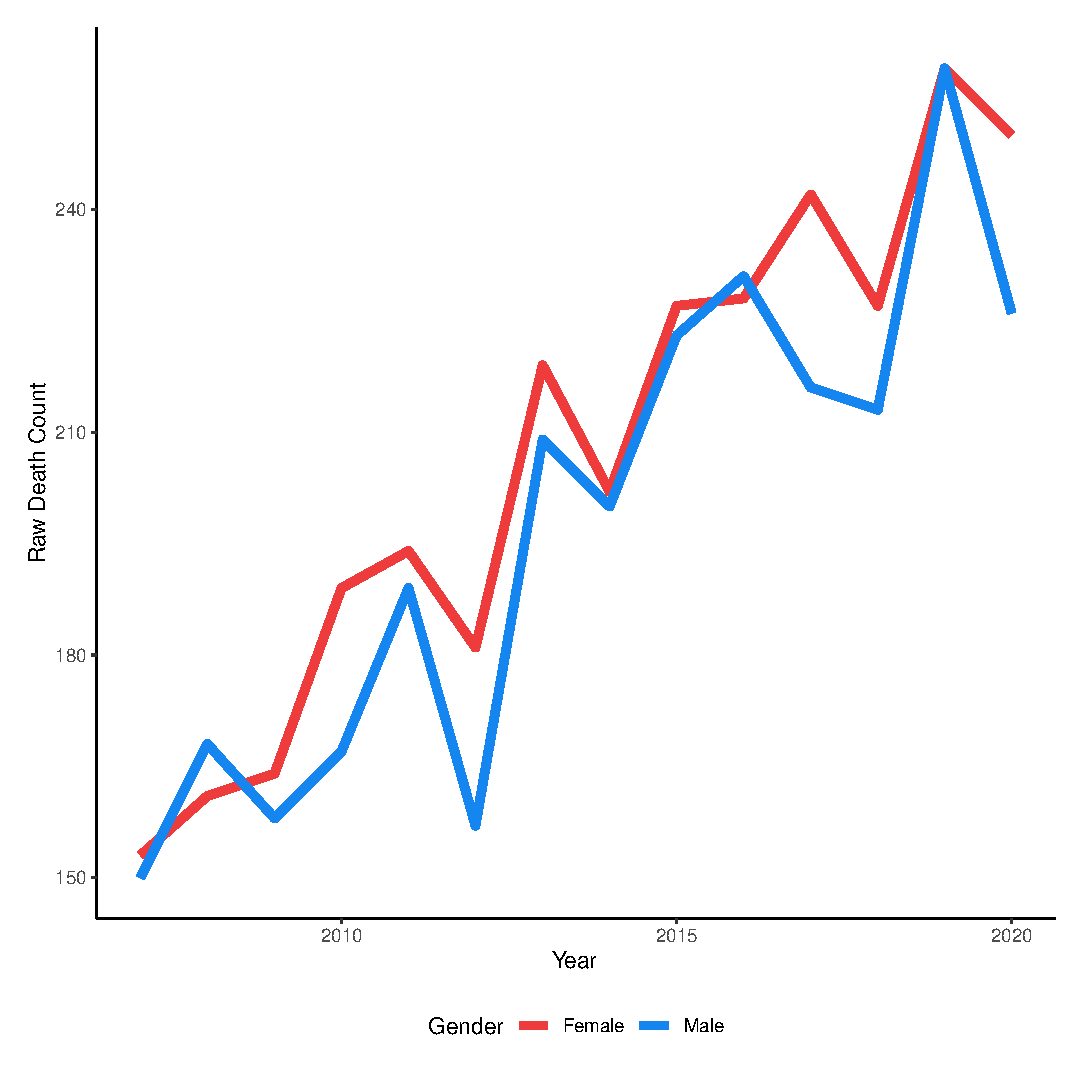
\includegraphics[scale=0.5]{analysis/output/raw_deaths_by_gender_plot.eps}
    \caption{Figure \textbf{a}: Crude Number of Deaths: Male, Female}
    \label{fig:crude_deaths_by_gender}
\end{figure}

\begin{figure}
    \centering
    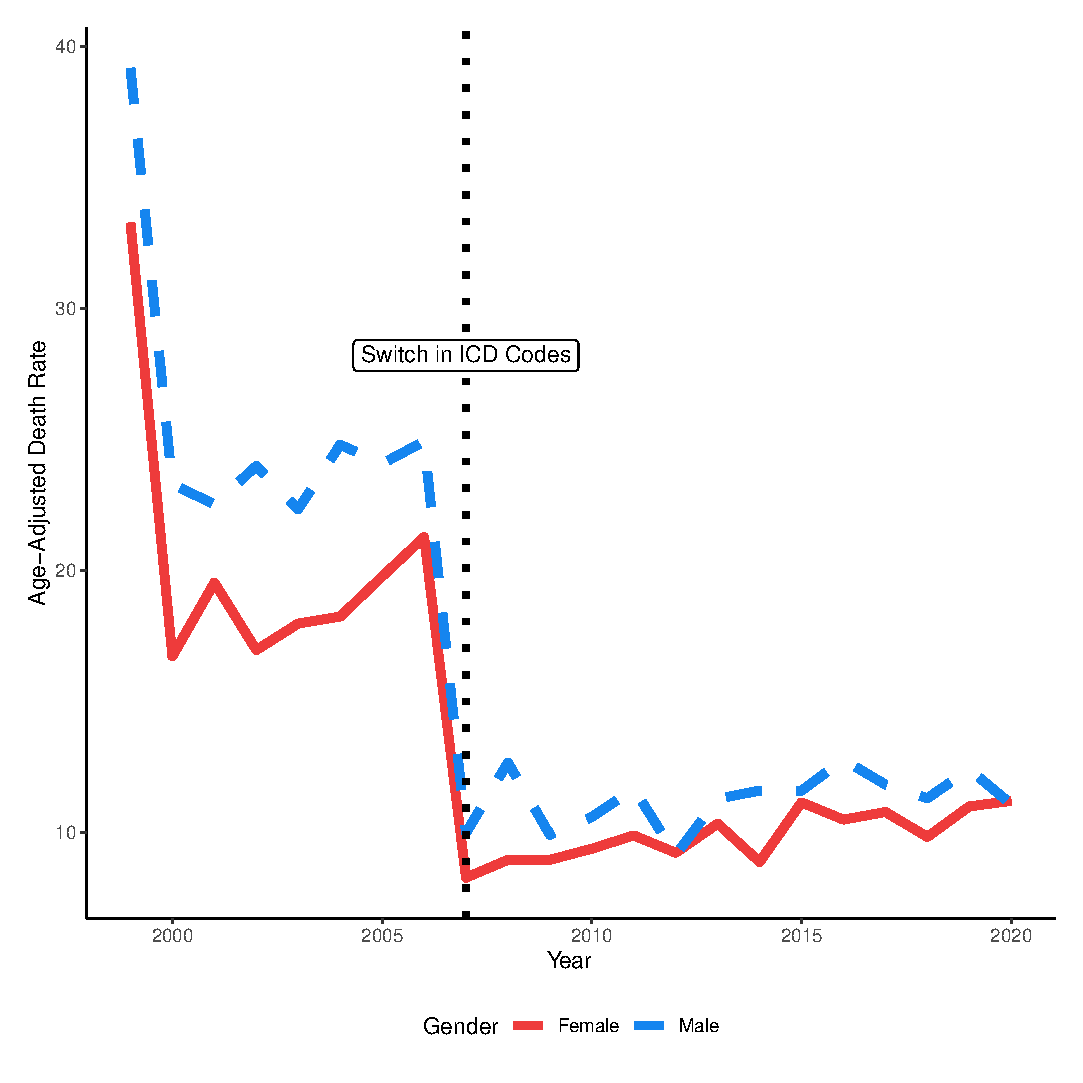
\includegraphics[scale=0.5]{analysis/output/age_adj_deaths_by_gender_plot.eps}
    \caption{Figure \textbf{b}: Age-Adjusted Mortality: Male, Female}
    \label{fig:age_adj_deaths_by_gender}
\end{figure}


\begin{figure}
    \centering
    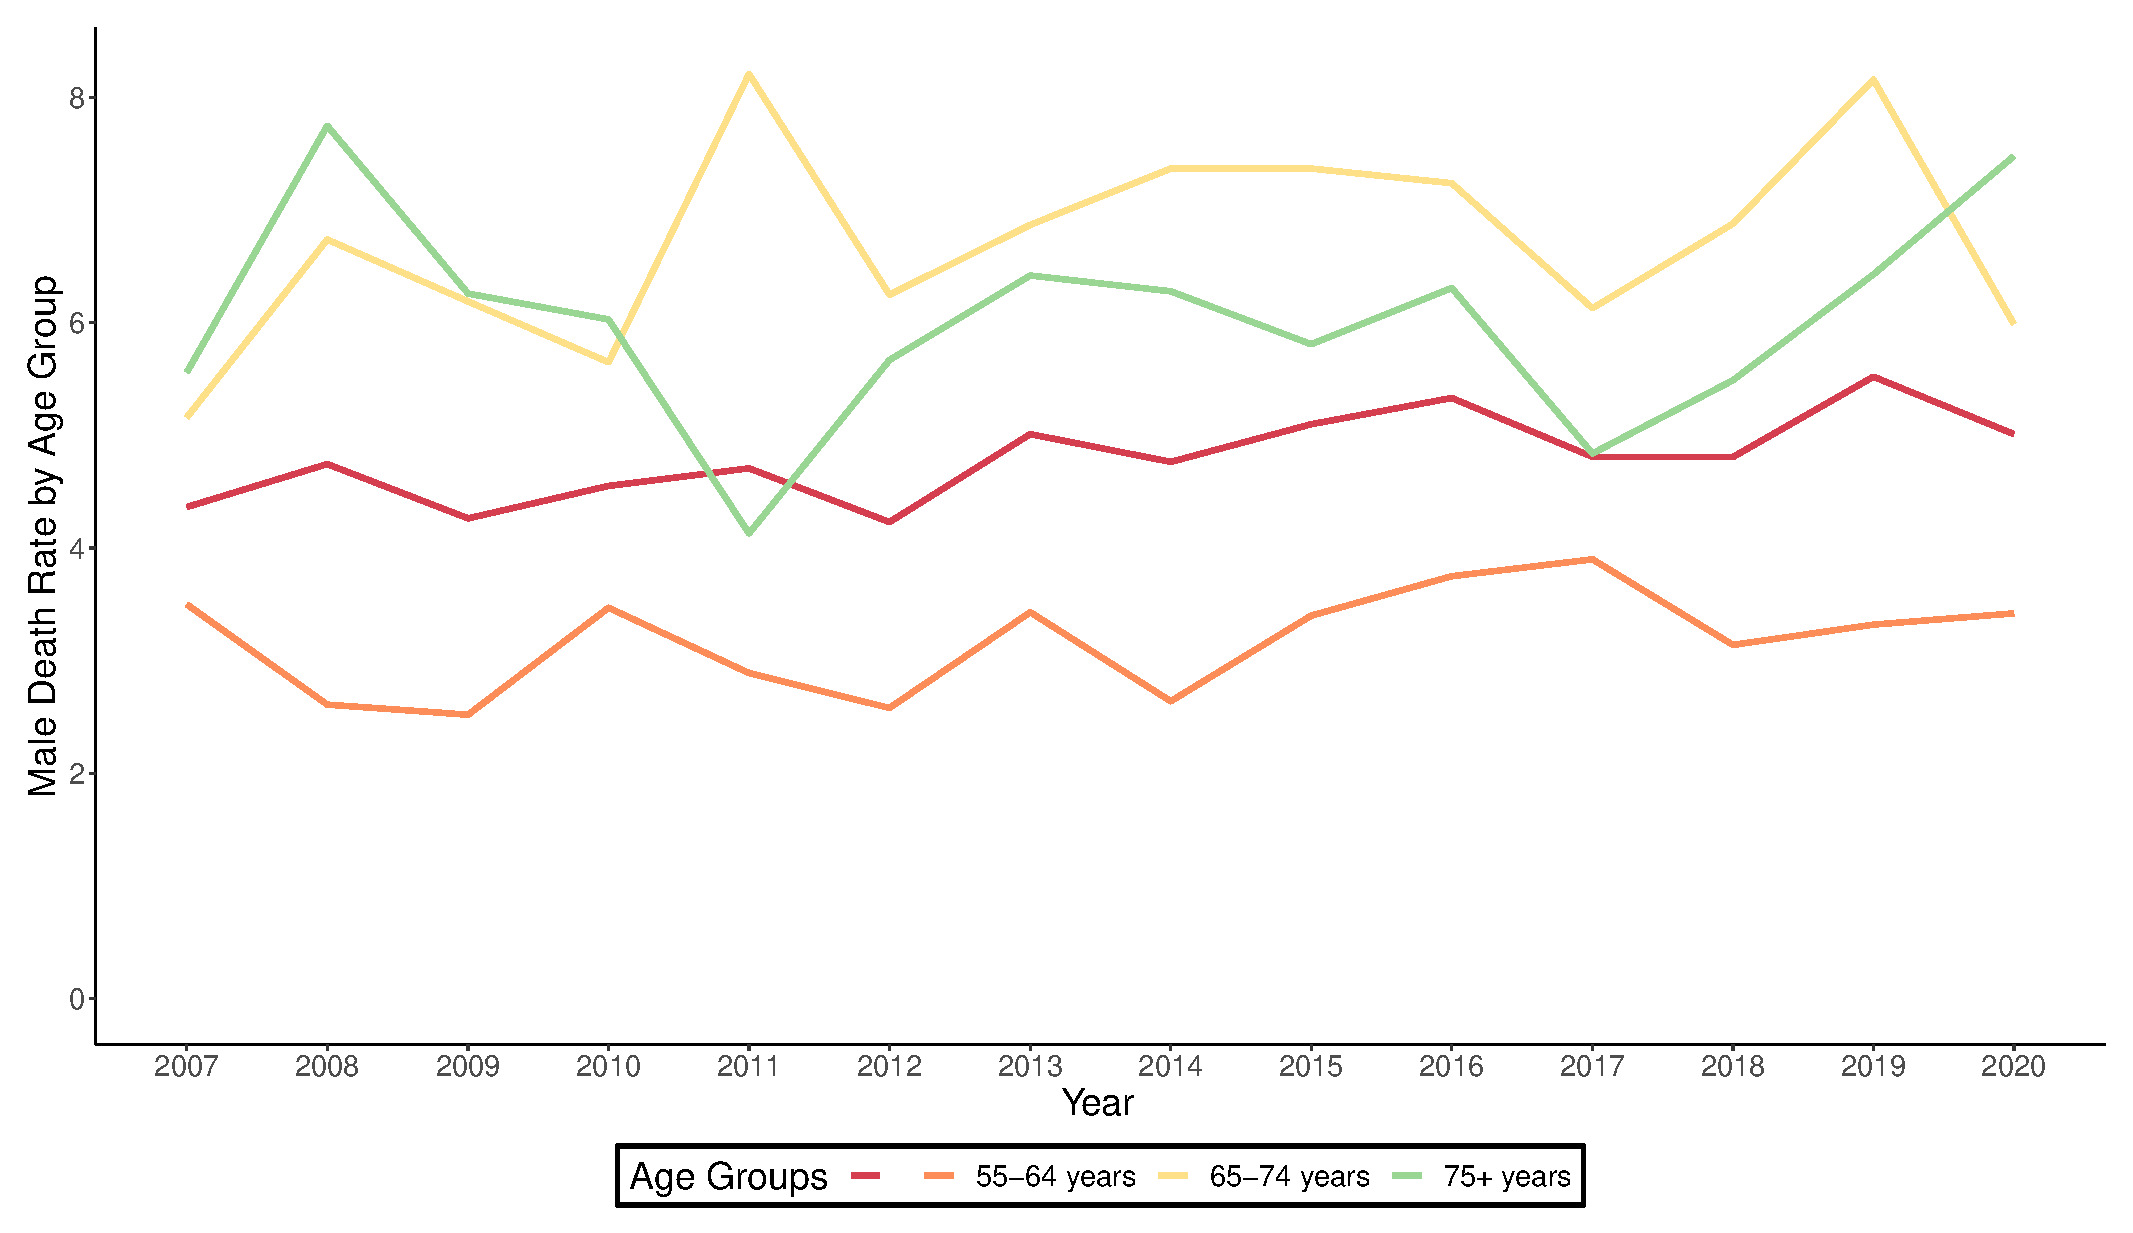
\includegraphics[scale=0.5]{analysis/output/male_age_specific_deaths_plot.eps}
    \caption{Figure \textbf{c}: Age-Specific Mortality: Male}
    \label{fig:male_age_specific_deaths}
\end{figure}

\begin{figure}
    \centering
    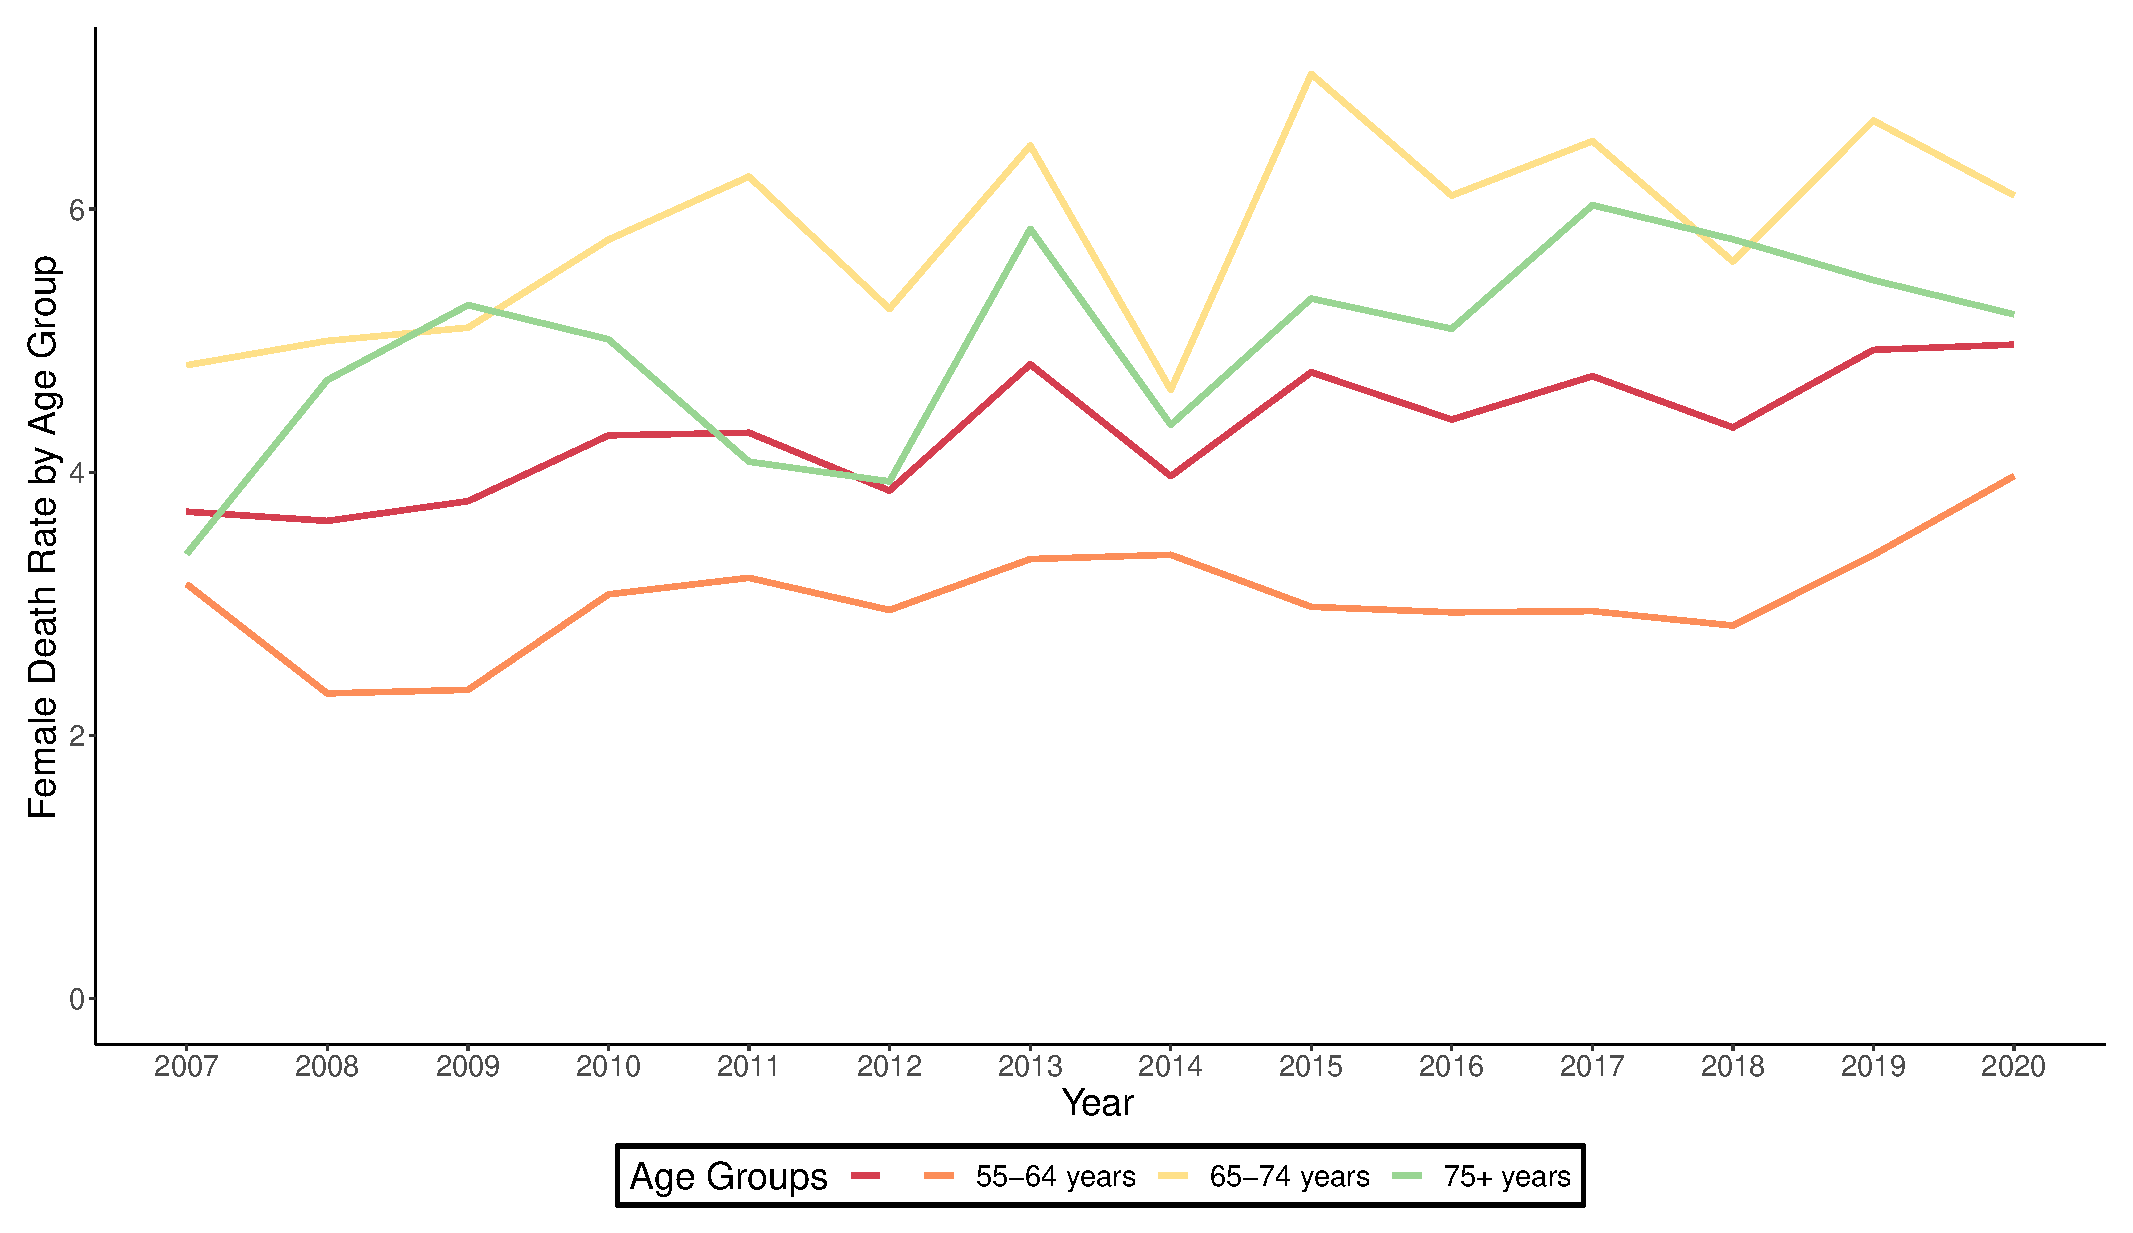
\includegraphics[scale=0.5]{analysis/output/female_age_specific_deaths_plot.eps}
    \caption{Figure \textbf{d}: Age-Specific Mortality: Female}
    \label{fig:female_age_specific_deaths}
\end{figure}

TODO: Table 1.

\section*{Discussion}
 
\par \bigskip
\noindent Our findings demonstrate that the incidence of CJD has risen considerably in recent years in the US, disproportionately affecting older patients and female patients. These results align closely with recent data from Japan and may be largely attributed to demographic changes in recent years.4 Our study’s main limitation is a reliance on death certificate data for estimating CJD incidence.

\par \bigskip
\noindent This data may be subject to miscoding or misdiagnosis, though existing research supports the use of death certificates for understanding CJD epidemiology.6 This analysis underscores the changing landscape of CJD in the US in recent years and suggests a need for close surveillance among the aging US population.  


% Bibliography
\bibliographystyle{paper/paper/Science}
\bibliography{paper/paper/deactivation_bib}


\end{document}



